\documentclass[aps,prb,twocolumn,superscriptaddress,preprintnumbers,amsmath,amssymb,floatfix]{revtex4}
%\documentclass[aps,prb,preprint,superscriptaddress,amsmath,amssymb,floatfix]{revtex4}
%\documentclass[aps,prl,onecolumn,groupedaddress,amsmath,amssymb,12pt]{revtex4}
\usepackage{graphicx}
\usepackage{ifthen}
\usepackage{dcolumn}% Align table columns on decimal point
\usepackage{bm}% bold math
\usepackage{multirow}
\usepackage{booktabs}
\usepackage{bm}% bold math
\usepackage{amsbsy}
\usepackage{amsmath}
\usepackage{amssymb}
\usepackage{subfigure}


%Definition of new commands
\newcommand{\f}[2]{\ensuremath{\frac{\displaystyle{#1}}{\displaystyle{#2}}}}
\newcommand{\lr}[1]{\langle{#1}\rangle}
\newcommand{\colv}[2] {\left(\begin{array}{c} #1 \\ #2 \end{array}\right)}
\renewcommand{\thefootnote}{\fnsymbol{footnote}}
\newcommand{\be} {\begin{eqnarray}}
\newcommand{\ee} {\end{eqnarray}}
%--------------------------------------------------------------------------
%EQ COMMANDS
%--------------------------------------------------------------------------
\newcommand{\two}{\mspace{-2.0mu}}
\newcommand{\four}{\mspace{-4.0mu}}
\newcommand{\plus}{\mspace{-4.5mu}+\mspace{-3.5mu}}
\newcommand{\minus}{\mspace{-4.5mu}-\mspace{-3.5mu}}
\newcommand{\pp}{'\mspace{-2.0mu}'}
\newcommand{\xlb}[4]{#1\ifthenelse{\equal{#2}{0}}{}{_{\alpha #2}}
\mspace{-2.0mu}\genfrac{(}{)}{0pt}{1}{\ifthenelse{\equal{#3}{0}}{0}{l #3}} 
{\ifthenelse{\equal{#4}{0}}{0}{b #4}}}

\newcommand{\xkv}[4]{#1\mspace{-5.0mu}\left(\mspace{-8.0mu}
\begin{smallmatrix}#2\four{}\four{}\mspace{-8.0mu}&\pmb{\kappa}#3\\&\nu 
#4\end{smallmatrix}\mspace{-5.0mu}\right)}

\newcommand{\evect}[6]{#1\mspace{-4.0mu}\left(\mspace{-8.0mu}
\begin{smallmatrix}#2\mspace{-8.0mu}&\pmb{\kappa} #3 &b #5\\&\nu #4 &
\alpha #6\end{smallmatrix}\mspace{-5.0mu}\right)}

\newcommand{\varmat}[8]{\mspace{-5.0mu}\left(\mspace{-8.0mu}
\begin{smallmatrix}\ifthenelse{\equal{#3}{0}}{\mspace{-8.0mu}&b_{#1}&b_{#2}
\\&\alpha_{#1}&\alpha_{#2}} {\ifthenelse{\equal{#7}{0}}{#1\mspace{-8.0mu}&
\pmb{\kappa}#2#3\mspace{-8.0mu}&\pmb{\kappa}#4#5\mspace{-8.0mu}&\pmb{\kappa}
#6\\&\nu#2&\nu#4&\nu#6} {#1\mspace{-8.0mu}&\pmb{\kappa}#2#3\mspace{-8.0mu}&
\pmb{\kappa}#4#5\mspace{-8.0mu}&\pmb{\kappa}#6#7\mspace{-8.0mu}&\pmb{\kappa}
#8\\&\nu#2&\nu#4&\nu#6&\nu#8}}\end{smallmatrix}\mspace{-5.0mu}\right)}

\newcommand{\EXP}[1]{\exp\mspace{-5.0mu}\left[#1\right]\mspace{-3.0mu}}

\newcommand{\tpp}[2]{\left(\mspace{-2.0mu}\xkv{\omega}{}{}{}#1\xkv{\omega}
{}{'}{'}#2\xkv{\omega}{}{\pp}{\pp}\mspace{-2.0mu}\right)}



%--------------------------------------------------------------------------
\newcommand{\SUM}[2]{\ifthenelse{\equal{#1}{0}}{\sum_{
\alpha_{#2},b_{#2},l_{#2}}^{3,n,N}} {\ifthenelse{\equal{#1}{1}}{\sum_{
\alpha_{#2},b_{#2}}^{3,n}}{\sum_{\pmb{\kappa}#2,\nu#2}^{N,3n}}}}

\newcommand{\SUMprime}[2]{\ifthenelse{\equal{#1}{0}}
{\sum_{\alpha_{#2},b_{#2},l_{#2}}^{3,n,N}} 
{\ifthenelse{\equal{#1}{1}}{\sum_{\alpha_{#2},b_{#2}}^{3,n}}
{\sum_{\pmb{\kappa}^{'}#2,\nu#2}^{N,3n}}}}

\newcommand{\SUMalpha}[2]{\ifthenelse{\equal{#1}{0}}
{\sum_{\alpha_{#2}}^{3}} {\ifthenelse{\equal{#1}{1}}
{\sum_{\alpha_{#2},b_{#2}}^{3,n}}{\sum_{\pmb{\kappa}#2,\nu#2}^{N,3n}}}}
%--------------------------------------------------------------------------
\newcommand{\SUMalphap}[2]{\ifthenelse{\equal{#1}{0}}
{\sum_{\alpha'_{#2}}^{3}} {\ifthenelse{\equal{#1}{1}}
{\sum_{\alpha'_{#2},b'_{#2}}^{3,n}}{\sum_{\pmb{\kappa}#2,\nu#2}^{N,3n}}}}

\newcommand{\SUMb}[2]{\ifthenelse{\equal{#1}{0}}{\sum_{b_{#2}}^{n}}
 {\ifthenelse{\equal{#1}{1}}{\sum_{\alpha_{#2},b_{#2}}^{3,n}}
{\sum_{\pmb{\kappa}#2,\nu#2}^{N,3n}}}}

\newcommand{\SUMbp}[2]{\ifthenelse{\equal{#1}{0}}{\sum_{b'_{#2}}^{n}}
 {\ifthenelse{\equal{#1}{1}}{\sum_{\alpha'_{#2},b'_{#2}}^{3,n}}
{\sum_{\pmb{\kappa}#2,\nu#2}^{N,3n}}}}

\newcommand{\SUMl}[2]{\ifthenelse{\equal{#1}{0}}{\sum_{l_{#2}}^{N}}
 {\ifthenelse{\equal{#1}{1}}{\sum_{\alpha_{#2},b_{#2}}^{3,n}}
{\sum_{\pmb{\kappa}#2,\nu#2}^{N,3n}}}}

\newcommand{\SUMlp}[2]{\ifthenelse{\equal{#1}{0}}{\sum_{l'_{#2}}^{N}}
 {\ifthenelse{\equal{#1}{1}}{\sum_{\alpha'_{#2},b'_{#2}}^{3,n}}
{\sum_{\pmb{\kappa}#2,\nu#2}^{N,3n}}}}

\newcommand{\abcdt}[5]{\mspace{-4.0mu}\left(\mspace{-8.0mu}
\begin{smallmatrix}&\ifthenelse{\equal{#1}{}}{a}{#1}&\ifthenelse
{\equal{#3}{}}{c}{#3}\\&\ifthenelse{\equal{#2}{}}{b}{#2}&\ifthenelse
{\equal{#4}{}}{d}{#4}\end{smallmatrix}\mspace{-2.0mu};\ifthenelse
{\equal{#5}{}}{t}{#5}\right)}

\newcommand{\abcd}[4]{\mspace{-4.0mu}\left(\mspace{-8.0mu}
\begin{smallmatrix}&\ifthenelse{\equal{#1}{}}{a}{#1}&\ifthenelse
{\equal{#3}{}}{c}{#3}\\&\ifthenelse{\equal{#2}{}}{b}{#2}&\ifthenelse
{\equal{#4}{}}{d}{#4}\end{smallmatrix}\mspace{-3.0mu}\right)}

\newcommand{\abt}[3]{\mspace{-4.0mu}\left(\mspace{-8.0mu}\begin
{smallmatrix}&\ifthenelse{\equal{#1}{}}{a}{#1} \\&\ifthenelse{
\equal{#2}{}}{b}{#2}\end{smallmatrix}\mspace{-2.0mu};
\ifthenelse{\equal{#3}{}}{t}{#3}\right)}

\newcommand{\ab}[2]{\mspace{-4.0mu}\left(\mspace{-8.0mu}
\begin{smallmatrix}&\ifthenelse{\equal{#1}{}}{a}{#1} \\&\ifthenelse
{\equal{#2}{}}{b}{#2}\end{smallmatrix}\mspace{-3.0mu}\right)}

\newcommand{\kvbat}{\mspace{-4.0mu}\left(\mspace{-8.0mu}
\begin{smallmatrix} &\pmb{\kappa} &b \\ &\nu &\alpha\end{smallmatrix}
\mspace{-2.0mu};t\right)}
%--------------------------------------------------------------------------
\newcommand{\kvbatp}{\mspace{-4.0mu}\left(\mspace{-8.0mu}
\begin{smallmatrix} &\pmb{\kappa} &b' \\ &\nu &\alpha'\end{smallmatrix}
\mspace{-2.0mu};t\right)}

\newcommand{\kvbaw}{\mspace{-4.0mu}\left(\mspace{-8.0mu}
\begin{smallmatrix} &\pmb{\kappa} &b \\ &\nu &\alpha\end{smallmatrix}
\mspace{-2.0mu};\omega\right)}

\newcommand{\kvbawp}{\mspace{-4.0mu}\left(\mspace{-8.0mu}
\begin{smallmatrix} &\pmb{\kappa} &b' \\ &\nu &\alpha'\end{smallmatrix}
\mspace{-2.0mu};\omega\right)}

\newcommand{\kvba}{\mspace{-4.0mu}\left(\mspace{-8.0mu}
\begin{smallmatrix} &\pmb{\kappa} &b \\ &\nu &\alpha\end{smallmatrix}
\mspace{-3.0mu}\right)}

\newcommand{\kvbap}{\mspace{-4.0mu}\left(\mspace{-8.0mu}
\begin{smallmatrix} &\pmb{\kappa}' &b \\ &\nu' &\alpha\end{smallmatrix}
\mspace{-3.0mu}\right)}
%--------------------------------------------------------------------------
\newcommand{\kpvba}{\mspace{-4.0mu}\left(\mspace{-8.0mu}
\begin{smallmatrix} &\pmb{\kappa}^{'} &b \\ &\nu &\alpha\end{smallmatrix}
\mspace{-3.0mu}\right)}

\newcommand{\kva}{\mspace{-4.0mu}\left(\mspace{-8.0mu}
\begin{smallmatrix} &\pmb{\kappa} \\ &\nu &\alpha\end{smallmatrix}
\mspace{-3.0mu}\right)}

\newcommand{\kvap}{\mspace{-4.0mu}\left(\mspace{-8.0mu}
\begin{smallmatrix} &\pmb{\kappa} \\ &\nu &\alpha'\end{smallmatrix}
\mspace{-3.0mu}\right)}

\newcommand{\kvb}{\mspace{-4.0mu}\left(\mspace{-8.0mu}
\begin{smallmatrix} &\pmb{\kappa} &b \\ &\nu \end{smallmatrix}
\mspace{-3.0mu}\right)}

\newcommand{\kvbp}{\mspace{-4.0mu}\left(\mspace{-8.0mu}
\begin{smallmatrix} &\pmb{\kappa} &b' \\ &\nu \end{smallmatrix}
\mspace{-3.0mu}\right)}

\newcommand{\kvt}{\mspace{-4.0mu}\left(\mspace{-8.0mu}
\begin{smallmatrix}&\pmb{\kappa} \\&\nu\end{smallmatrix}
\mspace{-2.0mu};t\right)}

\newcommand{\kvzero}{\mspace{-4.0mu}\left(\mspace{-8.0mu}
\begin{smallmatrix}&\pmb{\kappa} \\&\nu\end{smallmatrix}
\mspace{-2.0mu};0\right)}

\newcommand{\kpvt}{\mspace{-4.0mu}\left(\mspace{-8.0mu}
\begin{smallmatrix}&\pmb{\kappa}^{'} \\&\nu\end{smallmatrix}
\mspace{-2.0mu};t\right)}

\newcommand{\kvw}{\mspace{-4.0mu}\left(\mspace{-8.0mu}
\begin{smallmatrix}&\pmb{\kappa} \\&\nu\end{smallmatrix}
\mspace{-2.0mu};\omega\right)}

\newcommand{\kv}{\mspace{-4.0mu}\left(\mspace{-8.0mu}
\begin{smallmatrix}&\pmb{\kappa} \\&\nu\end{smallmatrix}
\mspace{-3.0mu}\right)}

\newcommand{\kvp}{\mspace{-4.0mu}\left(\mspace{-8.0mu}
\begin{smallmatrix}&\pmb{\kappa'} \\&\nu'\end{smallmatrix}
\mspace{-3.0mu}\right)}

\newcommand{\kw}{\mspace{-4.0mu}\left(\mspace{-8.0mu}
\begin{smallmatrix}&\pmb{\kappa} \\&\omega\end{smallmatrix}
\mspace{-3.0mu}\right)}

\newcommand{\kpvp}{\mspace{-4.0mu}\left(\mspace{-8.0mu}
\begin{smallmatrix}&\pmb{\kappa'} \\&\nu'\end{smallmatrix}
\mspace{-3.0mu}\right)}
%--------------------------------------------------------------------------
\newcommand{\lbt}{\mspace{-4.0mu}\left(\mspace{-8.0mu}
\begin{smallmatrix}&l \\&b\end{smallmatrix}\mspace{-2.0mu};t\right)}

\newcommand{\lbtp}{\mspace{-4.0mu}\left(\mspace{-8.0mu}
\begin{smallmatrix}&l' \\&b'\end{smallmatrix}\mspace{-2.0mu};t\right)}

\newcommand{\lt}{\mspace{-4.0mu}\left(\mspace{-8.0mu}
\begin{smallmatrix}&l\end{smallmatrix}\mspace{-2.0mu};t\right)}

\newcommand{\ltp}{\mspace{-4.0mu}\left(\mspace{-8.0mu}
\begin{smallmatrix}&l'\end{smallmatrix}\mspace{-2.0mu};t\right)}

\newcommand{\lb}{\mspace{-4.0mu}\left(\mspace{-8.0mu}
\begin{smallmatrix}&l \\&b\end{smallmatrix}\mspace{-3.0mu}\right)}

\newcommand{\lbp}{\mspace{-4.0mu}\left(\mspace{-8.0mu}
\begin{smallmatrix}&l' \\&b'\end{smallmatrix}\mspace{-3.0mu}\right)}
%--------------------------------------------------------------------------
%COMMANDS
%--------------------------------------------------------------------------

%--------------------------------------------------------------------------
\begin{document}
%--------------------------------------------------------------------------

%--------------------------------------------------------------------------
\title{Evaluation of the Virtual Crystal Approximation for Predicting 
Thermal Conductivity}
%--------------------------------------------------------------------------
\author{Jason M. Larkin}
\affiliation{Department of Mechanical Engineering\\Carnegie Mellon 
University\\Pittsburgh, PA 15213}
\author{A. J. H. McGaughey}
\email{mcgaughey@cmu.edu}
\affiliation{Department of Mechanical Engineering\\
Carnegie Mellon University\\Pittsburgh, PA 15213}
%--------------------------------------------------------------------------

%--------------------------------------------------------------------------
\date{\today}
%--------------------------------------------------------------------------


%--------------------------------------------------------------------------
\begin{abstract}
%--------------------------------------------------------------------------
Accurately predicting the thermal conductivity of a dielectric or 
semiconducting material requires the properties of phonons from the entire 
Brillouin zone. Accurate predictions of phonon properties for bulk systems 
can be made with anharmonic lattice dynamics theory using ab initio 
calculations. However, computational costs limit the size of unit cells 
in ab initio calculations to be less than 100 atoms, making it difficult 
to directly incorporate the effects of disorder. Alternatively, theory 
that treats disorder as a harmonic perturbation can be used to estimate 
the reduction in phonon lifetimes due to disorder scattering without 
the use of a large unit cell. Under this approximation, the disordered
 crystal is replaced with a perfect “virtual crystal” with properties 
equivalent to an averaging over the disorder (e.g.  mass or bond 
strength). 
In this work, the virtual crystal approximation for mass disorder is 
evaluated by examining two model alloy systems: Lennard-Jones argon 
and Stillinger-Weber silicon. In both cases the perfect crystal is 
alloyed with a heavier mass species up to equal concentration . These 
two alloyed systems have different ranges of phonon frequencies, 
lifetimes, and mean free paths. For Stillinger-Weber silicon, the 
virtual crystal approximation predicts phonon properties and thermal 
conductivity in good agreement with molecular dynamics-based methods. 
For Lennard-Jones argon, the virtual crystal approximation underpredicts 
the high frequency phonon lifetimes, leading to an underpredicting of 
its thermal conductivity.
%--------------------------------------------------------------------------
\end{abstract}
%--------------------------------------------------------------------------


%--------------------------------------------------------------------------
\maketitle
%--------------------------------------------------------------------------
\clearpage
%--------------------------------------------------------------------------
\section{\label{S:Intro}Introduction}
%--------------------------------------------------------------------------

For thermolectric device applications, minimizing a thermoelectric 
material's thermal 
conductivity has become a promising technique for increasing $ZT>3$.
\cite{chen_recent_2003,dresselhaus_new_2007} In semiconductor alloys, 
understanding the effect of disorder is necessary for optimizing 
ZT by further lowering thermal conductivity.
\cite{he_thermoelectric_2006,huang_filler-reduced_2010,
toberer_phonon_2011,tian_phonon_2012}

Abeles first introduced the idea of using a virtual crystal (VC) to 
replace a disordered one by treating both
disorder and anharmonicity as perturbations.\cite{abeles_lattice_1963} 

Many experimental results and trends in thermal conductivity 
of a range of materials 
can be explained using the VC approximation.  
However, a complete 
description of the thermal transpot in alloys requires modeling intrinsic 
and 
disordered scattering to predict phonon lifetimes.

Modeling phonon lifetimes is usually done by treating both intrinsic 
and disordered scattering as pertubations under the VC approximation. 
The relative simplictiy 
of this approach allows the use of compuatioanlly expensive ab-initio 
methods. Recently, work using ab-initio calculations, anharmonic 
lattice dynamics (ALD) and the VC 
approximation to predict phonon mode frequencies, lifetimes and 
group velocities of materials with realtively
large\cite{garg_role_2011,lindsay_thermal_2012} 
moderate \cite{thermal_shiomi_2011}, and 
small \cite{tian_phonon_2012} 
thermal conductivities. However, no comprehensive study has been performed 
to assess the applicability of this perturbative approach for a range 
of heavily disorered systems using multiple predictive methods.


The goal of this work is to verify the use of the virtual crystal 
approximation for predicting thermal conductivity by a detailed comparison 
of 3 predictive methods: MD-based normal mode 
decomposition (NMD) and green-kubo (GK), 
and anharmonic lattice dynamics (ALD) which treats the harmonic and 
anharmonic phonon scattering as perturbations. When used with the VC 
approximation, these methods are referred to as VC-NMD and VC-ALD.
Two model alloy systems 
with mass defects ($m^a_{1-c}m^b_{c}$) are considered: 
Lennard-Jones (LJ) argon and Stillinger-Weber (SW) silicon. 
In both cases the perfect crystal is 
alloyed with a heavier mass species up to equal concentration, spanning 
range of perturbative to heavy disorder. These 
two alloyed systems have very different ranges of phonon frequencies, 
lifetimes, group velocities and total thermal conuctivity. 
For Stillinger-Weber silicon, 
VC-ALD predicts phonon properties and thermal VC-NMD and GK. 
For Lennard-Jones argon, the VC-ALD approximation underpredicts 
the high frequency phonon lifetimes, leading to an underpredicting of 
its thermal conductivity. The different thermal conductivity spectra of 
the modeled 
and the breakdown of the perturbative scattering models are examined.

%--------------------------------------------------------------------------
\section{\label{S:}Virtual Crystal (VC) Approximation}
%--------------------------------------------------------------------------
Abeles introduced the idea of using a virtual (perfect) crystal 
to replace a disordered one, computing the
thermal conductivity of Si/Ge alloys by treating both
disorder and anharmonicity as perturbations.
\cite{abeles_lattice_1963} 
We calculate at all compositions of mass variation ($m^a_{1-c}m^b_{c}$)
the phonon modes of the virtual crystal (which has
a temperature dependent lattice parameter, mass, and
force constants of that particular composition)
and derive from the frequencies (Section ), 
group velocities (Section ),
and lifetimes (Section ) to calculate thermal
conductivity (Section ).

Many experimental results and trends in thermal conductivity 
of a range of materials 
can be explained using the VC approximation.  

Based on lattice dynamics 
calculations, the sound speed in simple alloys follows a simple scaling 
with mass or bulk modulus (spring constant) of the virtual crystal (see 
Section ). This is one exaplanation for the decreased thermal 
conductivity of germanium versus silicon. However, a complete 
description of the thermal transpot in alloys requires modeling intrinsic 
and 
disordered scattering (lifetimes) of phonons.

Cahill shows that conductivty of dilute Ge-doped Si epitaxial layers
agrees with 
a virtual crystal approximation with a phonon lifetime term that 
treats the defects as a peturbation (see section).
\cite{cahill_thermal_2004} 
Garg used ab initio calculations with anharmonic lattice dynamics (ALD) 
and the virtual crystal 
approximation (referred to as VC-ALD) 
to predict the thermal conductivity of Si-Ge alloys 
for all concentrations, obtaining good agreement with experiment.
\cite{garg_role_2011}  
A detailed study of PbTe/PbSe systems demonstrate the importance 
of bond environment for alloys.\cite{tian_phonon_2012} 

The computaitonal studies discussed above were limited to the use 
of VC-ALD because of the computational cost of ab initio calcualtions. 
Using empirical potentials, we study the effects of explicit 
disorder in the following sections.

%--------------------------------------------------------------------------
\subsection{\label{S:Lifetimes}Kinetic Theory}
%--------------------------------------------------------------------------

For a perfect system, all vibrational modes are phonons.

Using the single-mode relaxation
time approximation \cite{ziman_electrons_2001} as an approximate solution of
the Boltzmann transport equation \cite{peierls_quantum_2001} gives

\begin{equation}\label{EQ:M:k_mode}
\begin{split}
k_{vib,\mathbf{n}}=&\sum_{\pmb{\kappa}} \sum_\nu c_{ph}\kv 
\pmb{v}^{2}_{g,\mathbf{n}}\kv \tau\kv.
\end{split}
\end{equation}

Here, $c_{ph}$ is the phonon volumetric specific heat and 
${v}_{g,\mathbf{n}}$ is
the component of the group velocity vector in direction $\mathbf{n}$. 
Since the systems we consider are classical and obey Maxwell-Boltzmann 
statistics,\cite{mcquarrie_statistical_2000} the
specific heat is $k_{B}/V$ per mode in the harmonic limit where $V$ 
is the system volume. This approximation is used for all calculations 
in this work so that direct comparisons can be made for all predictions. 

Each mode contributing to the thermal conductivity has a frequency  
$\omega\kv$, which is related to the energy of a phonon in this mode 
by $\hbar\omega\kv$. In a perfect system, the allowed energies 
(frequencies) are eigenvalues of the system's Dynamical matrix, 
$D\kv$, which relates the mode eigenvector ($e\kvba$) 
and eigenvalue by
\begin{equation}\label{EQ:M:k_mode}
D\kv e\kvba = \omega\kv^2e\kvba.
\end{equation}

In a crystal all vibrational modes are plane-waves and as such 
can be identified by a unique wave-vector 
$\mathbf{\kappa}$, eigenvector $e\kvba$, and a possibly 
degenerate frequency $\omega\kv$. In a disordered structure, such as a 
crystal lattice with randomly arranged and differing mass species, 
all vibrational modes exist at the wavevector $[000]$. In general, 
these disordered vibrational modes will not be pure plane-waves and 
will be non-degenerate in frequency. We examine 


It thus becomes difficult to predict an 
effective dispersion 

%--------------------------------------------------------------------------
\subsection{\label{S:}Phonon Group Velocities}
%--------------------------------------------------------------------------
The group velocity vector is the gradient of the dispersion curves 
(i.e., $\partial \omega / \partial \pmb{\kappa}$), which can be 
calculated from the frequencies and wavevectors using finite differences. 
In this work, the group velocities are calculated using finite difference 
and quasi-harmonic lattice dynamics because a very small finite difference 
can be used which reduces the error.\cite{mcgaughey2006b} 

Of particular interest if the phonon mean free path (MFP),

\begin{equation}\label{EQ:M:phonon_mfp}
\begin{split}
\Lambda\kv = |\pmb{v}_{g}| \tau\kv,
\end{split}
\end{equation}

which requires a group velocity.

In ordered systems, the group velocity generally scales with both the 
density and stiffness of the material. For example, 
the reduced vibrational conductivity of Ge compared to Si can 
be (partially) explained in both in terms of the $\bar m$ 
(germanium has a larger density $\rho$ than silicon) 
and the group velocity (germanium has a smaller bulk modulus $B$, 
and $v_g \propto \sqrt{B/\rho}$.
Thus, for alloys, there should also be a corrsponding scaling 
of the group velocity with the alloy's concentration (mass
density).


%--------------------------------------------------------------------------
\subsection{\label{S:}VC and Gamma DOS Comparison}
%--------------------------------------------------------------------------

The low frequency

Similar agreement at low frequencies was found in ab initio predictions 
for $Si_cGe_{1-c}$.\cite{garg_role_2011} Bouchard show that 
alloy DOS at 
low frequency varies smoothly with concentration for 
a-$Si_cGe_{1-c}$.\cite{bouchard_vibrational_1988} 

The frequencies of the Gamme point modes are shifted slighty higher 
because of the explicit use of atoms of lighter mass than the virtual 
mass.

%--------------------------------------------------------------------------
\begin{figure}
\begin{center}
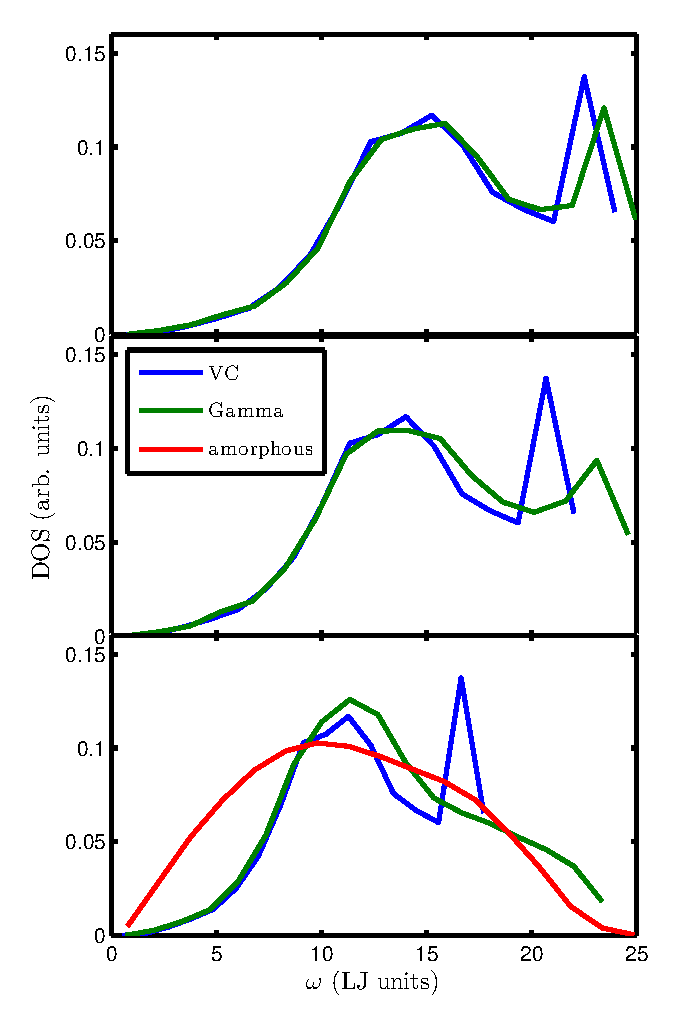
\includegraphics[scale=0.7]
{/home/jason/disorder/lj/alloy/lj_alloy_dos_c05-5_3.eps}
\vspace*{-5mm}
\end{center}
\caption{\label{FIG:phonon_diff} virtual crystal results}
\end{figure}
%--------------------------------------------------------------------------

%--------------------------------------------------------------------------
\subsection{\label{S:}Structure Factor of Gamma Point Modes}
%--------------------------------------------------------------------------

\begin{equation}\label{EQ:M:EL}
E^L\kv = 
\left|
\sum_{l,b} 
\hat{\mathbf{\kappa}} \cdot e\kvba 
\EXP{i\pmb{\kappa}\cdot\mathbf{r}_0\ab{l}{b}} 
\right|^2
\end{equation}

\begin{equation}\label{EQ:M:EL}
E^T\kv = 
\left|
\sum_{l,b} 
\hat{\mathbf{\kappa}} \times e\kvba 
\EXP{i\pmb{\kappa}\cdot\mathbf{r}_0\ab{l}{b}} 
\right|^2
\end{equation}

\begin{equation}\label{EQ:M:SL}
S^{L,T}\kw = 
\sum_{\nu} E^{L,T}\kv
\delta (\omega-\omega\kv)
\end{equation}

Demonstrates the importance of dispersion, even along different lattice 
directions ([100 vs [111]) and polarizations ($S^L,T$).

With increasing concentration, the structure factor spreads in width,  
particularly at high frequencies.  The VC mass becomes larger and the 
peaks in the structure factor shift to lower frequencies. 
The peaks in the structure factor for Gamma point modes are shifted to 
slightly 
higher frequencies beacuse of the explicit use of masses less than the 
VC mass, and effect which can also be seen in the DOS comparisons 
(Fig ).

An effective dispersion can be extracted by locating the peaks in the 
structure factors, where the effects of polarization, virtual mass, and 
anisotropic dispersion can be observed (Fig. ). These well-defined peaks 
at all wavevectors is unique to the disordered lattice. 
Typically, the structure factor for amorphous materials have well-defined 
peaks only for small wavevector.(cite) The frequencies extracted from 
the structure factors agree with the VC predictions to less than 
5$\%$ at the highest frequencies. Because of this, 
we use the group velocities predicted by the VC dispersion  
in both our VC-NMD and VC-ALD calculations for 
consistency. 

Duda shows the reduction in group velocity of moderate to high 
frequency modes in a 1D alloy are drastically reduced by considering 
the effects of zone folding.\cite{duda_reducing_2011} 
Based on the structure factors in 
Fig. , the reduction due to zone folding 
seems to underpredict the group velocity of 
moderate to high frequency modes.

%--------------------------------------------------------------------------
\begin{figure}
\begin{center}
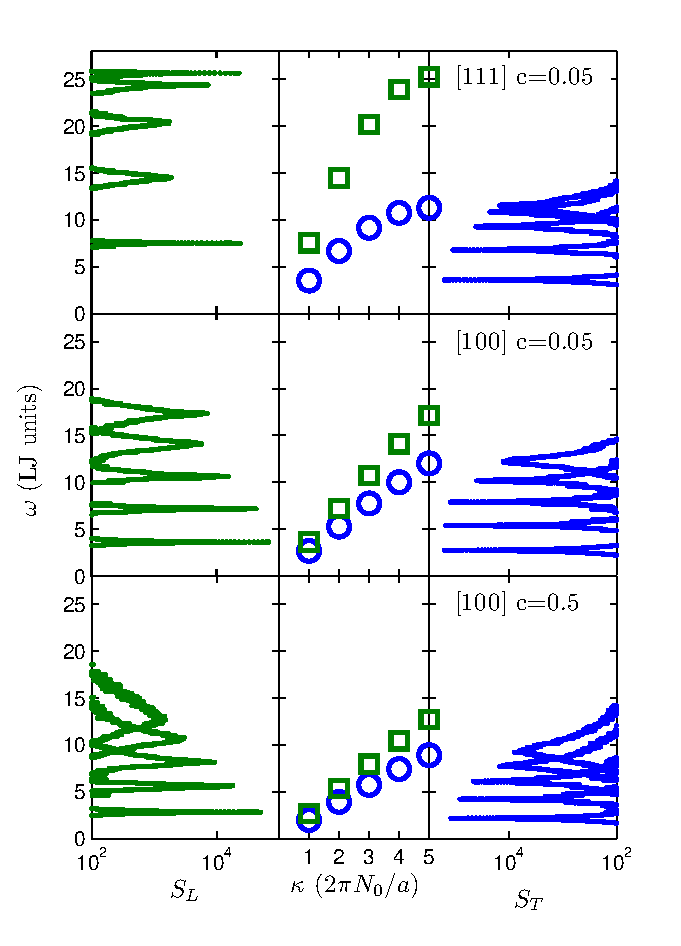
\includegraphics[scale=0.7]
{/home/jason/disorder/lj/alloy/lj_alloy_dsf_100_111.eps}
\vspace*{-5mm}
\end{center}
\caption{\label{FIG:phonon_diff} virtual crystal results}
\end{figure}
%--------------------------------------------------------------------------

%--------------------------------------------------------------------------
\subsection{\label{S:}Phonon Lifetimes}
%--------------------------------------------------------------------------

\begin{equation}\label{EQ:M:tau_matthiessen}
\frac{1}{\tau\kv} = \frac{1}{\tau_{p-p}\kv} + \frac{1}{\tau_{d}\kv},
\end{equation}
where $\tau_{p-p}\kv$ accounts for phonon-phonon scattering,
accounts for boundary scattering, $\tau_{d}\kv$ accounts for defect 
scattering.

Phonon-phonon scattering ($\tau_{p-p}\kv$) is typically treated 
using anharmonic perturbation theory including only 3-phonon 
processes.\cite{turney_predicting_2009,garg_role_2011,tian_phonon_2012} 
It has been estimated that the effects of higher order phonon 
processes are small \cite{ecsedy_thermal_1977}.
At low frequencies,
$\tau_{p-p}\kv$ follows a scaling due to both normal ($B_1\omega^2$) 
and umklapp ($B_2\omega^2$) 3-phonon scattering processes, where 
the density of states is Debye-like. The 
constants $B_1$ and $B_2$ are typically fit to experimental data.

Using harmonic perturbation theory, Tamura gives a general expression 
for mass point defect scattering \cite{tamura_isotope_1983}
\begin{equation}\label{EQ:M:tau_d}
\begin{split}
\frac{1}{\tau_{d}\kv} = \frac{\pi}{2N}\omega\kv^2 
\sum_{\mathbf{\kappa'}\nu'} \delta( \omega\kv - 
\omega\kvp ) \\
\sum_{b} g(b) 
|e^*\kvbap \cdot e\kvba |^2 ,
\end{split}
\end{equation}
where 
$g(b) = \sum_i c_i(b)(1-m_i(b)/\bar m(b))^2,$
N is the number of unit cells. and $c_i$ is the fraction, $m_i$ is the mass, 
and $\bar m_i$ is the average mass of the i-th species.

For the simple single species systems considered in this work, 
$\frac{1}{\tau_{d}\kv} =\frac{\pi}{2} g \omega\kv^2 D(\omega\kv)$, where 
$D(\omega\kv)$ is the density of states. Under the Debye-approximation, 
the phonon scattering due to mass point-defects 
is given by $A\omega^{-4}$, where $A$ is a constant related to the unit 
cell volume, branch-averaged group velocity, and disorder coupling strength 
($g$ in Eq. above). The frequency dependence ($\omega^4$) is the same as 
Rayleigh scattering, which is valid at low frequency where the Debye 
approximation is valid.

Bond disorder 
can be accounted for using a similar expression with an average
atomic radius or suitable scattering cross-section.
\cite{klemens_scattering_1955,klemens_thermal_1957} 
The effect of bond and mass disorder has been investigated computationally 
by Skye and 
Schelling for Si/Ge \cite{skye_thermal_2008}, 
where it was shown that mass disorder is 
the dominant scattering mechanism. In this work we consider only 
mass disorder.

While the
expression for harmonic defect scattering (Eq.) is valid for
perturbative disorder, its use leads to good agreement with
several experimental and computational results with large disorder.  
Cahill shows that conductivty reduction in dilute 
Ge-doped Si epitaxial layers 
is captured by mass perturbative disorder.\cite{cahill_thermal_2005} 
In this case, the mass disorder is large ($m_{Ge}/m_{Si} = 2.6$) 
but the overall disorder strength is dictated by the concentration. 
For example, as little as $6.2\times10^{19} cm^{-3}$ Ge
($g = 3.1\times10^{-3}$) is enough to reduce the thermal conductivity of 
Si by almost a factor of 2.\cite{cahill_thermal_2004}
Even in the
case of the $Ni_{0.55}Pd_{0.45}$ alloy, the atomic species
are chemically similar but both the mass disorder 
($m_{Pd}/m_{Ni} \approx 2$) and concentration are large ($g=0.078$) 
and good agreement is seen with the Eq..
\cite{kamitakahara_vibrations_1974}

Computational results for moderate to high thermal conductivity 
alloys show good to excellent agreement with experimental results
\cite{thermal_shiomi_2011,garg_role_2011,lindsay_thermal_2012}.
Compuational results for small thermal conductivirty alloys 
show universal trends but little experimental results are 
available for comparison.


%--------------------------------------------------------------------------
\subsection{\label{S:}Phonon Lifetime Predictions}
%--------------------------------------------------------------------------

%--------------------------------------------------------------------------
\subsubsection{\label{S:Lifetimes}Normal Mode Decomposition (NMD)}
%--------------------------------------------------------------------------

As an alternative to VC-ALD models for predicting phonon lifetimes, 
we also use the normal mode decomposition (NMD) method. NMD maps the 
atomic coodinates (position and velocities) of all atoms in an MD 
simulation onto vibrational normal modes.(cite) The vibrational mode 
frequencies ($\omega\kv$) and eigenvectors ($e\kvba$) are necessary 
for the mapping. The vibrational normal mode coordinates, 
$q\kvt and qdot\kvt$, are required 
to calculate the total vibrational normal mode energy $E\kv(t)$.

The phonon lifetime is predicted using 

\begin{equation}\label{EQ:M:tau_d}
\tau\kv = \int_{0}^{\infty} \frac{<E\kvt E\kvzero>}{ <E\kvzero E\kvzero> }dt.
\end{equation}

This is necessary for the disordered systems where spectral NMD\cite{} 
can produce multiple peaks in an isolated mode's 
power spectrum. 
This feature is not surprising given two considerations: 1) the MD simulations 
contain explicit disorder which incluences the atomic trajectories 2)
the normal modes are mapped without using the exact eigenvectors and 
frequencies of the explicitly disordered system (see Fig. and ).

Under the VC approximation, the phonon eigenvectors 
are those of pure plane-waves by definition. 
In a disordered supercell, the vibrational 
modes are not pure plane-waves (phonons) (see Section) and exist at the 
Gamma point ([000]). Lifetimes NMD and Gamma-NMD, are examined in Section 
and referred



%--------------------------------------------------------------------------
\subsection{\label{S:Lifetimes}VC-NMD and Gamma Phonon Lifetimes}
%--------------------------------------------------------------------------

%--------------------------------------------------------------------------
\begin{figure}
\begin{center}
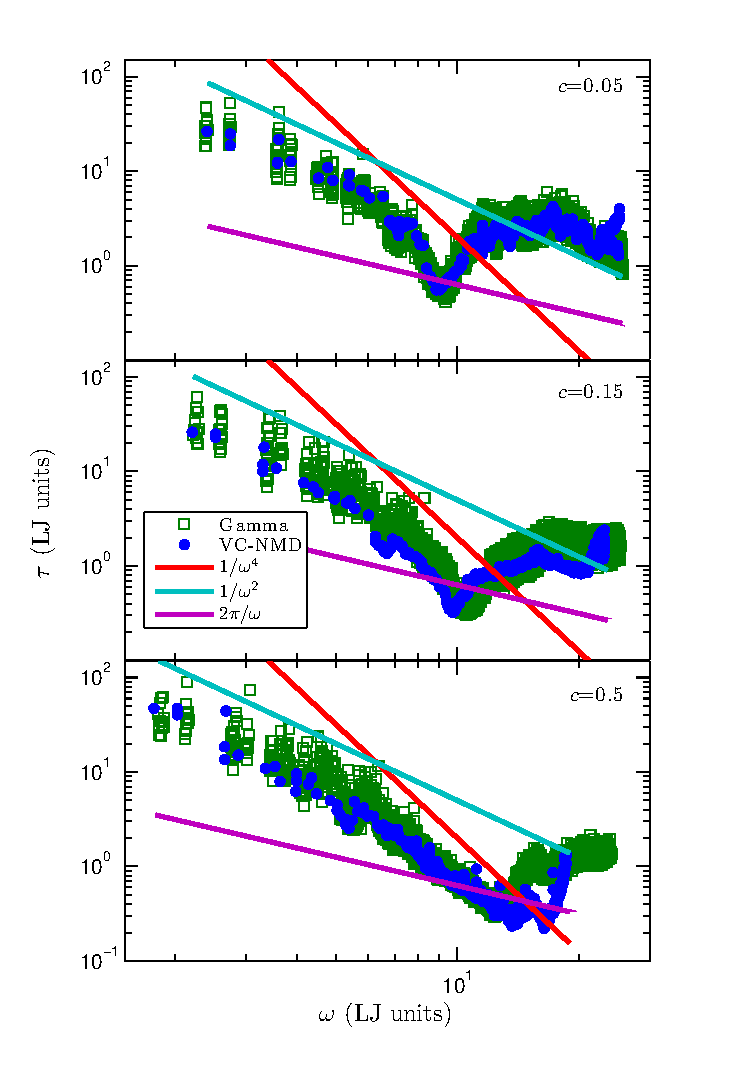
\includegraphics[scale=0.7]
{/home/jason/disorder/lj/alloy/lj_alloy_nmd_vc_gamma_life.eps}
\vspace*{-5mm}
\end{center}
\caption{\label{FIG:phonon_diff} virtual crystal results}
\end{figure}
%--------------------------------------------------------------------------

Gamma refers to mapping using the eigenvectors of the exact harmonic 
eigenmdoes of the disordered supercell. 

For VC-NMD, the normal mode mappings are performed using eigenvectors 
which are plane waves.\cite{}

eigenvector mappings \cite{koker_thermal_2009}
\cite{qiu_molecular_2011} use NMD to predict the phonon properties of 
PbTe using a classical model.
\cite{shiomi_thermal_2011} half-huesler usese $\Phi'$ and ALD, find good 
agreement. \cite{thomas_predicting_2010} finds increased scattering in 
water-filled CNTs. \cite{ong_reduction_2011} finds increased scattering 
of phonons in CNTs on a substrate. 

In these studies, the atomic coordinates are being mapped onto modes which 
are not eigenmodes of the system's Hamiltonian. Still, the spectral widths 
(inverse lifetimes) of these mappings contain information about the 
scattering time scales associated with these modes.   

Previous 
studies have used the spectral NMD using exact and 
non-exact mode eigenvectors to extract mode timescales.(cite) 
The lifetimes using these mappings 
contain the effects of both intrinsic(cite) and disorder scattering(cite).
Interpretation 
of these timescales as phonon lifetimes has led to succesful thermal 
conductivity predictions in a range of ordered and disordered materials.
(cite)
Given the possible ambiguity of the lifetimes predicted using VC-NMD, 
it is necessary  
to compare the predicted thermal conductivities using a range of methods 
which posses no such ambiguity (such as VC-ALD and GK, see Section ). 

%--------------------------------------------------------------------------
\subsection{\label{S:}Vibrational Mode Diffusivity}
%--------------------------------------------------------------------------

In the classical limit where the specific heat $c_p\kv = k_{B}$, 
a vibrational mode's contribution to thermal 
conductivity is determined by that mode's thermal diffusivity. For 
phonons, the thermal diffusivity is simply 
\begin{equation}\label{EQ:M:k_HS}
D_{ph}(\omega\kv) = \pmb{v}^{2}_{g,\mathbf{n}}\kv \tau\kv.
\end{equation}
In heavily disordered systems, such as large $c$ alloys or glasses, 
modes can transport heat by harmonic coupling due to the disorder 
in the Allen-Feldman (AF) theory.(cite) With sufficient disorder, the 
harmonic AF theory is capable of accurately predicting a finite 
thermal conductivity.(cite shenogin, FKAW) In the classical limit, 
the AF thermal 
conductivity is written as
\begin{equation}\label{EQ:M:k_HS}
k_{AF} = \sum_\omega  \frac{k_{B}}{V} D_{AF}(\omega),
\end{equation}
where $V$ is the system volume and $D_{AF}(\omega_{AF})$ is the thermal 
diffusivity of the mode labeled by frequency 
$\omega_{AF} \equiv \omega\kv$, with 
$\nu$ ranging over all 
modes in the supercell and $\mathbf{\kappa} = [000]$.(cite) 

In the high-scatter (HS) limit, the AF diffusivity of each mode is
\begin{equation}\label{EQ:M:k_HS}
D_{AF,HS} = \frac{1}{3} v_s a.
\end{equation}
A similar HS limit for mode diffusivity 
is given by the Cahill-Pohl (CP) model, 
\begin{equation}\label{EQ:M:k_HS}
D_{CP,HS} = 0.403 v_s a.
\end{equation}
The CP thermal conductivity prediction in the HS limit is
\begin{equation}\label{EQ:M:k_HS}
k_{CP,HS} = (\frac{\pi}{6})^{1/3} (\frac{3}{2}) \frac{k_{B}}{V_b}b v_s a,
\end{equation}
where $V_b$ is the volume of the unit cell, $v_s$ is the 
branch-averaged sound speed, and $a$ is the lattice constant 
(or appropriate length scale).\cite{cahill_lattice_1988} 
Comparing with Eq., the AF,HS limit predicts a mode diffusivity and 
thermal conductivity which is $\%20$ smaller then 
CP,HS.\cite{cahill_lattice_1988} 
Ignoring this small difference, 
the interpretation for both $D_{AF,HS}$ and $D_{CP,HS}$ is of a vibrational 
mode with a group velocity equal to the sound speed 
and mean-free path equal to the 
lattice spacing. 

While the CP,HS model assumes $\tau = 1/\omega$ and $v_g = v_s$ for all 
modes, the AF theory is capable of predicting the mode diffusivities without 
any assumptions other than a harmonic approximation. 
Finite system size frequency spacings limit the $D_{AF}$ of the lowest 
frequency modes using the harmonic AF theory. In the infinite-size,  
low-frequency limt the AF conductivity of a disordered lattice is divergent 
due to lack of anharmonic phonon-phonon scattering.(cite)  
While the low frequency modes are not treated properly in the harmonic 
AF theory, 
$D_{AF}$ of high frequency modes in the heavily disordered ($c=0.5$) LJ 
alloy approaches that of similar frequency modes in the amorphous phase 
(Fig. ). 
In the amorphous phase, modes with significant 
contribution to thermal transport can be modeled using a mode-independent 
diffusivity of $D_{AF,HS}$ (Eq. ). In fact, the difference between  
$k_{AF} = 0.099 W/m=K$ and $k_{HS,CP} = 0.124$ is approximately 
$\%20$. 
This places a plausible lower-bound on the value of the phonon mode 
diffusivities, $D_{ph} \ge D_{AF,HS}$ predicted by VC-NMD and VC-ALD in 
the following section. In fact, thes

%--------------------------------------------------------------------------
\begin{figure}
\begin{center}
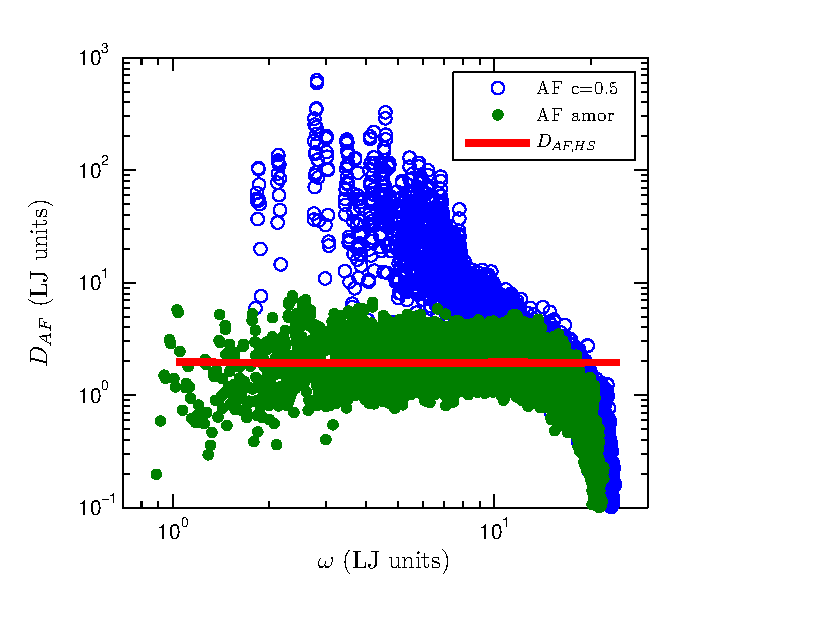
\includegraphics[scale=0.7]
{/home/jason/disorder/lj/alloy/af_c5_amor_DAF_kw_2.eps}
\vspace*{-5mm}
\end{center}
\caption{\label{FIG:phonon_diff} gamma point results}
\end{figure}
%--------------------------------------------------------------------------

%--------------------------------------------------------------------------
\subsection{\label{S:}VC-NMD and VC-ALD Mode Diffusivities}
%--------------------------------------------------------------------------

We now compare the phonon mode diffusitivies, $D_{ph}(\omega\kv)$
predicted by both VC-NMD and VC-ALD to the proposed lower limit 
$D_{AF,HS} = (1/3)v_sa$.  Here, $a$ is $1/2$ the lattice constant of the 
cubic conventional unit cells used for both FCC LJ argon and diamond-FCC 
SW silicon. 

For the VC-ALD method, 
the intrinsic $\tau\kv_{p-p}$ is calculated using the method described in.
\cite{turney_predicting_2009}
To calculate the disordered lifetimes (Eq. ), 
it is necessary to broaden 
the $\delta$ function using a Lorentzian function. 
For all calculations, the Lorentzian was broadened using a value of $100$ 
times the mean level spacing. The results do not differ significantly 
if this broadening value is varied by changing it manually or making 
the system size ($N_0$) bigger.

For LJ argon, VC-NMD predicts lifetimes which 
are generally larger than the period 
($2\pi/\omega\kv$)
of the vibrational oscillation (Ioffe-Regel limit)(cite), 
and actually increase with increasing 
frequency for small intervals (Fig. ). 
VC-NMD predicts larger phonon lifetimes at high 
frequency compared to VC-ALD (Fig. ) which predicts 
essentially monotonically 
decreasing lifetimes with increasing frequency. Because VC-NMD and VC-ALD 
use the same values for $c_{ph}\kv$ and $v_g\kv$, the phonon mode 
diffusivities $D_{ph}$ are also underpredicted by VC-ALD compared to VC-NMD. 
This leads to an 
underprediction for VC-ALD 
of both the thermal conductivity spectrum (Fig. ) at high 
frequency and the total thermal conductivity (Fig. ) compaed to VC-NMD. 

For both VC-NMD and VC-ALD, a significant number of modes have 
$D_{ph} \lt D_{AF,HS}$. This leads to an underprediction of the 
total thermal conducitvity compared to GK (Fig. ). The diffusivity of these 
modes can be adjusted such that any mode with $D_{ph} \lt D_{AF,HS}$ is 
given $D_{ph} = D_{AF,HS}$.  The results of this adjustment are examined 
in the next section.

%--------------------------------------------------------------------------
\begin{figure}
\begin{center}
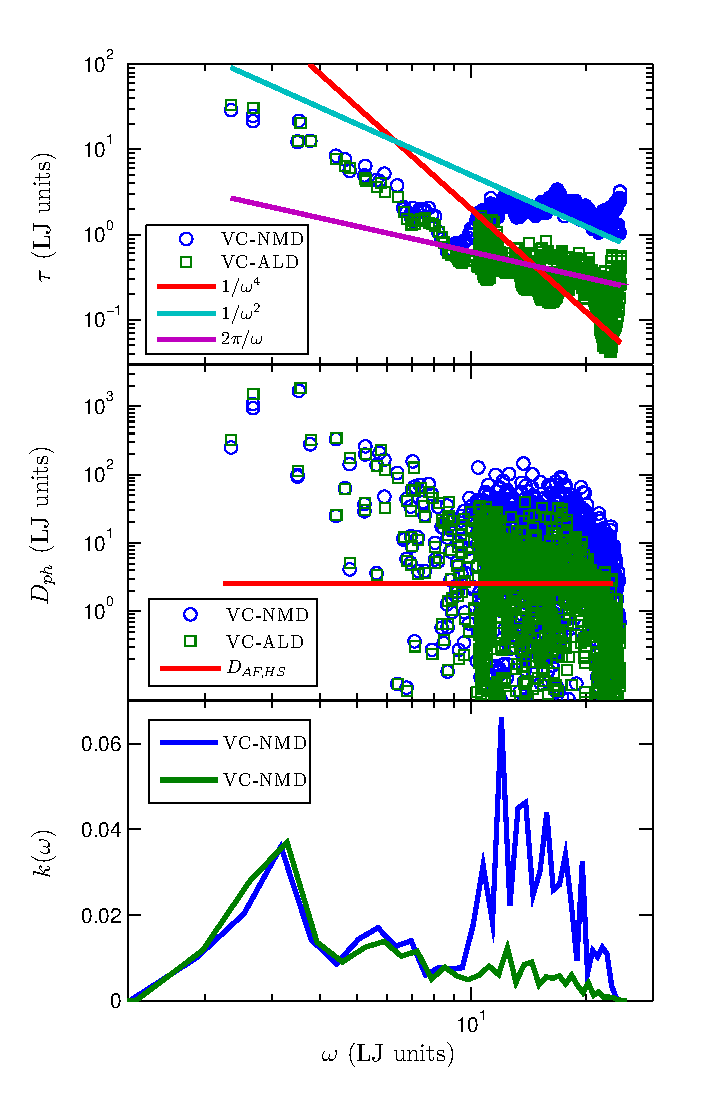
\includegraphics[scale=0.7]
{/home/jason/disorder/lj/alloy/af_nmd_ald_tau_diff_kw_c05_3.eps}
\vspace*{-5mm}
\end{center}
\caption{\label{FIG:phonon_diff} gamma point results}
\end{figure}
%--------------------------------------------------------------------------

%--------------------------------------------------------------------------
\begin{figure}
\begin{center}
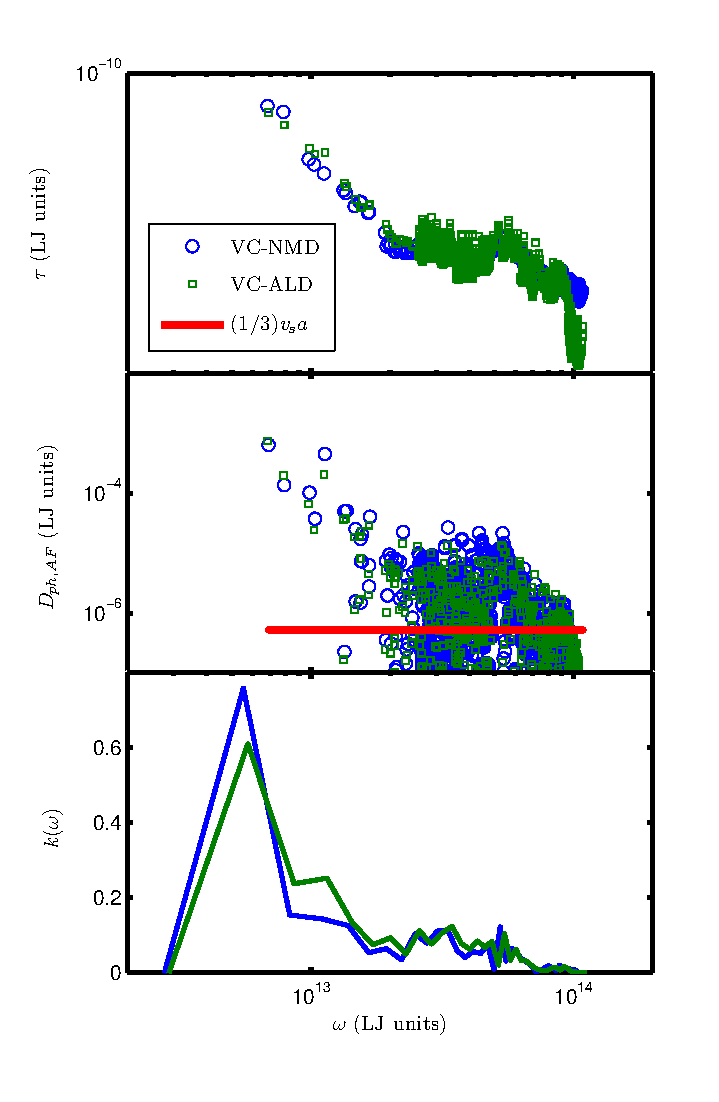
\includegraphics[scale=0.7]
{/home/jason/disorder/si/alloy/af_nmd_ald_tau_diff_kw_c05.eps}
\vspace*{-5mm}
\end{center}
\caption{\label{FIG:phonon_diff} gamma point results}
\end{figure}
%--------------------------------------------------------------------------

%--------------------------------------------------------------------------
\section{\label{S:Lifetimes}Thermal Conductivity Predictions}
%--------------------------------------------------------------------------
An addition of as little as 10\% Ge is sufficient to reduce the thermal 
conductivity to the minimum value achievable through alloying. 
Theoretically, mass disorder is found to increase the 
anharmonic scattering of phonons 
through a modification of their vibration eigenmodes. 
Notably, the thermal conductivity is found
to drop sharply after only a small amount of alloying. This
is due to the strong harmonic scattering of phonons even
in the dilute alloy limit.

Duda shows that taking a perfect alloy and disordering via an order 
parameter allows control of thermal conductivity.
\cite{duda_controlling_2012}

In fact, the beginning breakdown of the intrinsic scattering model 
($\tau_{p-p}\kw$) can be observed for the perfect ($c=0.0$) crystal at 
$T=40$ K (see Fig. ), where ALD begins to overpredict compared to GK.  This 
can be explained by the emerging importance of higher order (n$> 3$) 
n-phonon process at high temperatures.\cite{turney_predicting_2009}

For LJ argon, bulk thermal conductivity predictions are made for 
VC-NMD, VC-ALD and GK (Fig. ). For SW silicon, bulk thermal conductivity 
predictions can only be made for VC-ALD and GK (see Appendix ). 
For LJ argon, both VC-NMD and VC-ALD underpredict the thermal 
conductivity compared to GK. By adjusting



%--------------------------------------------------------------------------
\begin{figure}
\begin{center}
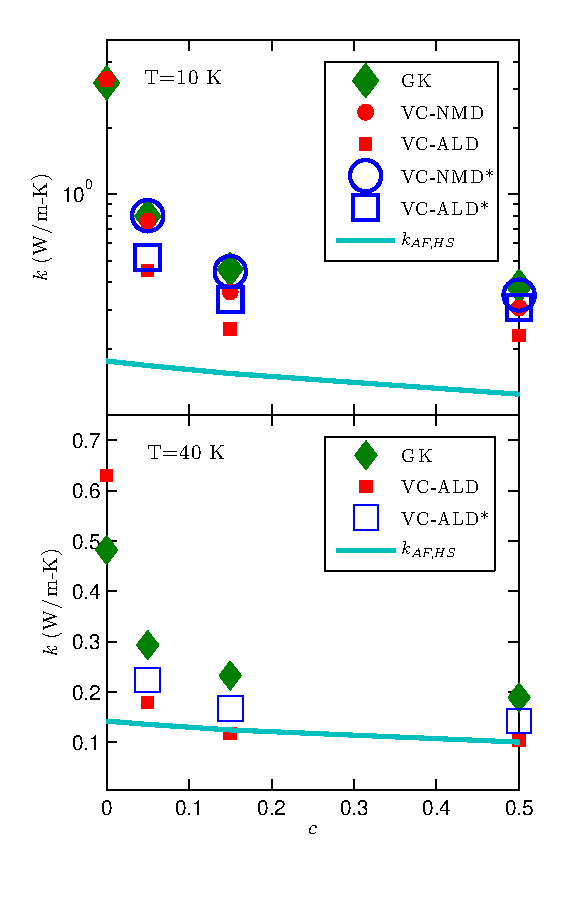
\includegraphics[scale=0.7]
{/home/jason/disorder/lj/alloy/lj_cond_compare.eps}
\vspace*{-5mm}
\end{center}
\caption{\label{FIG:gk_alloy} The vibrational conductivity of LJ alloys 
predicted using MD simulations and the Green-Kubo method. The predicted 
thermal conductivities are for a LJ alloy of the form $m^a_{1-c}m^b_{c}$, 
where $m^a =$ 1, $m^b=$ 3, and $m_r = m^a/m^b=$ 3 (in LJ units). As the 
alloy concentration is increased perturbatively, the vibrational 
conductivity drops quickly and saturates to a minimum at $c=0.5$. For 
$c=0.5$ the system is heavily disordered and the vibrational conductivity 
approaches that of an amorphous system.}
\end{figure}
%--------------------------------------------------------------------------

%--------------------------------------------------------------------------
\begin{figure}
\begin{center}
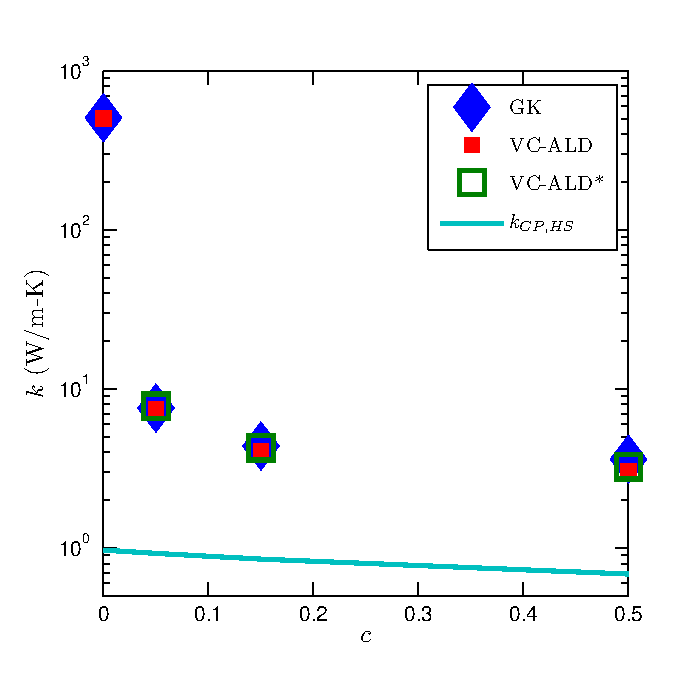
\includegraphics[scale=0.7]
{/home/jason/disorder/si/alloy/si_cond_compare.eps}
\vspace*{-5mm}
\end{center}
\caption{\label{FIG:gk_alloy} The vibrational conductivity of LJ alloys 
predicted using MD simulations and the Green-Kubo method. The predicted 
thermal conductivities are for a LJ alloy of the form $m^a_{1-c}m^b_{c}$, 
where $m^a =$ 1, $m^b=$ 3, and $m_r = m^a/m^b=$ 3 (in LJ units). As the 
alloy concentration is increased perturbatively, the vibrational 
conductivity drops quickly and saturates to a minimum at $c=0.5$. For 
$c=0.5$ the system is heavily disordered and the vibrational conductivity 
approaches that of an amorphous system.}
\end{figure}
%--------------------------------------------------------------------------

Experimental measurements of isotopically pure and Ge-doped 
Si epitaxial layers demonstrate the original theory by Abeles can predict 
thermal conductivity in dilute alloys. Abeles also found good agreement 
with dilute predictions for both experimental measurements of both 
Si-Ge alloys and also (Ga,In)As alloys.\cite{abeles_lattice_1963} However, 
both of these alloy systems have a relatively high thermal conductivities 
(on the order of 1-10 W/m-K at 300 K). However, in the heavily disordered 
system In(As,P) (mass ratio of 3.7) worse agreement with the Abeles theory 
is observed. 

The theory by Tamura is able to treat disorder scattering in an arbitrary 
crystal with dispersion. The theory, however, fails to predict the 
lifetimes of high-frequency modes, which are critical to the total 
thermal conductivity in LJ argon (see Fig. and ). To match the predicted 
phonon lifetime at high fequency for $c=0.05$ 
($\tau\kv \propto const.$, Fig. ), 
the Tamura theory requires a DOS which scales as 
$D(\omega\kv) \propto const.$. Clearly from Fig. , this is not the case 
with either the VC or Gamma modes. To match the predicted 
phonon lifetime at high fequency for $c=0.5$ 
($\tau\kv \propto 1/\omega\kv$, Fig. , also true for all $c$ in SW silicon), 

VC-NMD and VC-ALD underpredict vs GK by about 20-30, 
while for LJ the underprediction is 2-300

While Broido found that omission of optical scattering overpredicts the thermal 
conductivity of bulk Si by a factor of 2-3, 
optical modes contribute less than $5\%$ 
to thermal conductivity itself. Similarly, the diffusivity adjusted thermal 
cobductivities of SW Si are increased by less then $5\%$, demonstrating the 
unimportance of the high frequency ``optical'' modes in SW Si alloys.

%--------------------------------------------------------------------------
\section{\label{S:}Discussion}
%--------------------------------------------------------------------------

the problem is with taud.  VC-NMD agrees well with GK for both LJ and SW, 
while ALD-taud underpredcits for LJ.  VC-NMD and ALD-taud use the same 
group velocity and classical specific heat.

For diffusons, one can still assign a mfp by the following:

Particularly challenging is predicting a representative group velocity 
for modes in a disordered systems. 
Predicting a representative group velocity for modes in a disordered 
system is perhaps more important (and challenging) than predicting 
mode lifetimes. Use of the VC approximation is a theoretically and 
computationally simple way to predict a representative group velocity.

High thermal conductivity materials tend to have a conductivity spectrum 
which is peaked in the low frequency range.(cite) 
It is in this range where the mode 
lifetimes follow closely the scalings with frequency which can be 
predicted by treating intrinsic and disorder scattering as 
perturbations (Eq. ).

In contrast, 
in LJ argon the high frequency phonon mode properties are critical 
to the thermal transport.(cite)  
While the low frequency phonon properties predicted by VC-NMD and 
VC-ALD agree, it is the failure of the perturbative models at 
high frequency which causes VC-ALD to underpredict. The failure 
to account for harmonic disordered scattering due to the AF theory 
is responsible for causing both VC-NMD and VC-ALD to underpredict 
versus GK, which affects the high frequency modes significantly. 
LJ argon, with lower 
frequencies, lifetimes, and group velocities compared to 
``stiff'' SW silicon, 
is considered a ``soft'' system. The predictions using 
VC-NMD, VC-ALD demonstrate the importance of explicit disorder 
modeling in ``soft'' systems and possible underprediction 
of the thermal properties.\cite{tian_phonon_2012}

For SW silicon, the low frequency modes dominate thermal transport 
even in the heavily disordered alloy. 
It is thus unsurprising that predictions for 
SW silicon using VC-ALD agree well with VC-NMD and GK. This is also a 
plausible explanation for the success of predictions of using 
VC-ALD and ab initio calculations compared to experiment for 
``stiff'' systems Si-Ge, GaN, and Diamond.(cite) (cite new Hopkins)

In SW silicon even the amorphous phase has significant contributions 
from propagating modes which can be considered to be phonons. This is 
can seen by comparing the thermal conductivity predicted for the 
SW silicon amorphous phase ($k_{GK} =$ 2 W/m-K) compared to 
$k_{CP,HS} = $0.5 W/m-K.  For LJ argon in the amorphous phase, 
$k_{GK} = $0.121 W/m-K and $k_{CP,HS} =$ 0.12 W/m-K, indicating that 
all important modes to thermal transport are non-propagating.

%--------------------------------------------------------------------------
\subsection{\label{S:}Boundary Scattering}
%--------------------------------------------------------------------------
Boundary scattering is responsible for decreasing the long lifetimes 
(mean free paths) of low frequency phonons which carry a significant 
amount of heat, making it particularly e`ffective at decreasing the 
thermal conductivity of systems with length scale of 100s of nm and 
less.\cite{mcgaughey_nanostructure_2012}

First-principles calculations on some thermoelectric
materials show that phonons have a wide MFP distribution,
and hence relatively large nanostructures can reduce their
lattice thermal conductivity.5,18,19 On the other hand, recent
first-principles calculations have shown that the distribution is
much narrower for PbTe,20 and thus, further characterizations
of the distributions and the associated detailed heat conduction
of lead chalcogenides are important for better material design.
%--------------------------------------------------------------------------
\section{\label{S:}Summary}
%--------------------------------------------------------------------------


%--------------------------------------------------------------------------
\appendix
%--------------------------------------------------------------------------


\section{\label{A-Allowed-Wavevectors-Ordered}Allowed Wavevectors in 
Ordered and Disordered Systems}
%--------------------------------------------------------------------------
The phonon spectral energy is defined for the allowed wavevectors of a 
crystal, which can be specified from the crystal structure's Bravais 
lattice and its basis, i.e. unit cell. A $D$-dimensional Bravais lattice 
is a collection of points with
positions
\begin{equation}\label{crys_pos}
\begin{split}
\mathbf{u}_0\ab{l}{0} =& \sum^D_{\alpha} N_{\alpha}\mathbf{a}_{\alpha}
\end{split}
\end{equation}
where $N_{\alpha}$ and the summations if over the lattice vectors, 
$\mathbf{a}_{\alpha}$.\cite{ashcroft1976} The basis (or unit cell) is the 
building block of the crystal and they are arranged on the points defined 
by the Bravais lattice. The equillibrium position of any atom in the crystal 
can be described by
\begin{equation}\label{crys_pos2}
\begin{split}
\mathbf{u}_0\ab{l}{b} = \mathbf{u}_0\ab{l}{0} + \mathbf{u}_0\ab{0}{b}
\end{split}
\end{equation}
where $\mathbf{u}_0\ab{l}{0}$ is the equilibrium position of the 
$l^{\textrm{th}}$ unit cell and $\mathbf{u}_0\ab{0}{b}$ is the equilibrium 
position of the and $b^{\textrm{th}}$ atom in the unit cell relative to 
$\mathbf{u}_0\ab{l}{0}$.
For the LJ systems studied here, the cubic conventional cells are used with 
four atoms per unit cell.\cite{ashcroft1976} For our MD simulations, cubic 
simulation domains with periodic boundary conditions are used with 
$N_1 = N_2 = N_3 = N_0$.\cite{turney2009a,mcgaughey2004a} The allowed 
wavevectors for such crystal structures are
\begin{equation}\label{crys_pos3}
\begin{split}
\pmb{\kappa} = \sum_{\alpha} \mathbf{b}_{\alpha} 
\frac{n_{\alpha}}{N_{\alpha}},
\end{split}
\end{equation}
where $\mathbf{b}_{\alpha}$ are the reciprocal lattice 
vectors\cite{ashcroft1976} and $-N_{\alpha}/2 < n_{\alpha} 
\leq N_{\alpha}/2$, where $n_{\alpha}$ are integers and $N_{\alpha}$ 
are even integers.\cite{turney2009a} The wavevectors are taken to be 
in the first Brioullin zone.\cite{ashcroft1976}

Strictly speaking, the only allowed wavector in a disordered system is the 
gamma point ($\kappa = [0 0 0]$). As such, the lattice dynamics calculations 
are performed at the gamma point:

%--------------------------------------------------------------------------
\subsection{\label{S:Lifetimes:}Normal Mode Decomposition}
%--------------------------------------------------------------------------
If $\gamma \kv > \omega \kv$, then the vibrational mode is overdamped.  
Discuss why real-space method is necessary in this case.
%--------------------------------------------------------------------------
\section{\label{A-Finite-Sim}Finite Simulation-Size Scaling for Thermal 
Conductivity}
%--------------------------------------------------------------------------
To predict a bulk thermal conductivity, extrapolation is used by the 
following finite size scaling $ 1 / k \propto 1/N_0$. For VC-NMD and 
VC-ALD, the criteria for the validity of this finite size scaling 
is the low frequency modes in the finite system must be dominated by 
intrinsic scattering such that $\tau\kv \propto \omega\kv^{-2}$ 
and approximately follow the Debye approximation 
with respect to $v_{g,\mathbf{n}}$ and DOS $D(\omega\kv)$.(cite) For LJ 
argon, this requirement is satisfied for modest system sizes 
(up to $N_0 = 10$) so that both VC-NMD and VC-ALD predictions can be 
extrapolated to a bulk value. 
For SW silicon, the thermal conductivity is dominated by low-frequency 
modes. Becasue of this, large system sizes (up to $N_0 = 24$) are needed 
to satsify the 
extrpaolation requirement and only VC-ALD can be used.(cite) This 
underlines the computational efficieny of the VC-ALD method which is 
necessary when computationally expensive ab initio methods are used.
(cite) For the GK method, the finite size extrapolation is used for 
both LJ argon and SW silicon for smaller system sizes $N_0 \le 12$. 
The validity of this result can be explained in terms of a 
combination of effects which are specific to the MD simulations.
\cite{esfarjani_heat_2011}


\clearpage
\bibliographystyle{apsrev}
\bibliography{/home/jason/ntpl-ref/ntpl-jason/ntpl-jason-112412}
\end{document}
